\begin{figure}
\centering
\begin{tikzpicture}[->,>=stealth',auto,node distance=5cm,
    thick,
    main node/.style={circle,draw,font=\sffamily\Large\bfseries},
    aligned edge/.style={align=left}]

  \node[main node] (0) {$\location_0$};
  \node[main node] (1) [right of=0] {$\location_1$};

  \path[every node/.style={font=\sffamily\small}]
    (0) edge[aligned edge] node[above=0.2cm] {$t_0$} node[below=0.2cm] {$\update = \emph{id}$} (1)
    (1) edge[aligned edge, loop above] node[left=0.2cm] {$t_1$} node[right=0.2cm] {$\update(x) = x - 1$\\$\update(y) = y$\\$\guard = \braced{x > y}$} (1)
    ;
\end{tikzpicture}

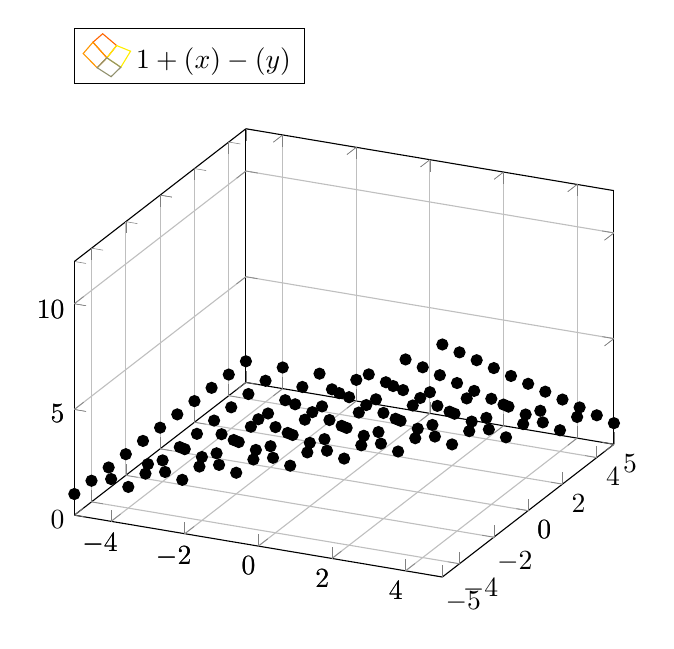
\begin{tikzpicture}
  \begin{axis}[
      extra x ticks={-4,-2,0,2,4},
      extra y ticks={-4,-2,0,2,4},
      extra z ticks={5,10},
      extra tick style={grid=major},
      legend style={
        at={(0,1.1)},
        anchor=south west
      },
    ]
    \addplot3 [
      unbounded coords=jump,
      mesh,
      shader=interp,
      samples at={-5,...,5},
      samples y={11},
      only marks,
    ] {1+max(x-y,0)};
    \addlegendentry{$1+\maxO{\ustate(x)-\lstate(y)}$}
  \end{axis}
\end{tikzpicture}
\hfil
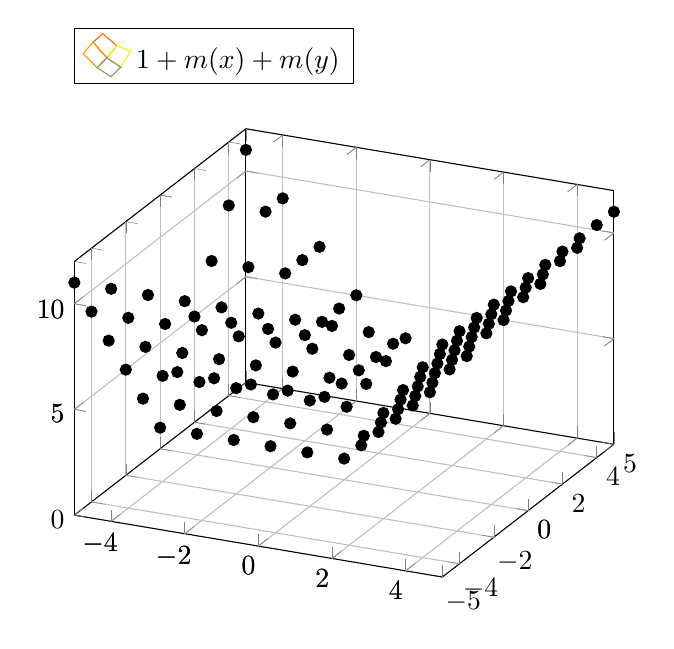
\begin{tikzpicture}
  \begin{axis}[
      extra x ticks={-4,-2,0,2,4},
      extra y ticks={-4,-2,0,2,4},
      extra z ticks={5,10},
      extra tick style={grid=major},
      legend style={
        at={(0,1.1)},
        anchor=south west
      },
    ]
    \addplot3 [
      unbounded coords=jump,
      mesh,
      shader=interp,
      samples at={-5,...,5},
      samples y={11},
      only marks,
    ] {1+abs(max(x,-y))+abs(max(x,-y))};
    \addlegendentry{$1+\abs{m(x)}+\abs{m(y)}$}
  \end{axis}
\end{tikzpicture}

\caption{Evaluation of the motivational example}
\label{fig:motivational_example}
\end{figure}
